\chapter{Literature Review}


\section{Abstract}

This chapter looks at existing research and development samples undertaken by other students from many countries around the world. These undertakings which have been published were sourced from publishing’s in academic papers, journal articles and books and gathered together from the major works to form part of the research of this narrow topic as they are in the same field of various implementations of random and automatic examination paper generation.


\section{Literature Review}

(Guang Cen, 2010) presented a method to eliminate (Mumbai, 2016) the tradition of the manual composition of examination papers which would usually rely on the writers’ own experience and style of question and knowledge. Although great care would be taken to achieve the best possible outcome of questions with traditional methods there was still the problem of a limited scope of topics and a time consideration. This would bring upon the separation between teaching and creating test papers by means of an automated computer system (Yang Yu, 2008). Comprised of JEE the test system includes modules such as user, subject, question, paper and classification management. Included in this is a question entry and generation module. These modules can be seen in Figure 1 – Schematic diagram of the system function module The question entry and generation makes use of browser and server architecture with a connection to a database of questions. Between this layer is a test server and a WWW server making up the middle layer (Chen, 2008). Figure 2 – Technology road-map of the system shows a flow chart of the system architecture and the use of the MVC pattern with a JSP view, Java Beans, Servlet Controller and a MySQL database (Liu, 2008). The page layout uses divs and CSS technology. In addition to this is support from JavaScript (R. Johnson, 2004). It is the browser which allows the user to choose the subject which they intend on examining. A question type such as student input and a difficulty level. With all these combined parameters, a paper is generated using the generation algorithm (Wang, 2008). This will then be stored in the test database which can be recalled at any stage through system functions for query, or to update the database and for maintenance. It runs in separated modes for user and administrator use. In the end the final document is processed into a Microsoft Word .doc file for distribution in an exam environment. From Figure 3 – Flow chart of the automatic paper generation method it shows how the document is generated.

There are 3 categories which this system falls under. They are, random algorithm based systems, backtracking systems and artificial intelligence and information processing. The first two do not satisfy the specifications (Guiying Deng, 1998). It is the latter which has been improved to avoid the disadvantages of the first and second algorithms. Giving it the ability of searching for questions based on experience and knowledge which guarantees a high standard and quality of examination papers (Hou, 2003). Through using a system with artificial intelligence and information processing the algorithm works quickly and effectively by not selecting a repeated question in a random manner. Questions and answers are separated. It also allowed the user a choice of topics, degree of difficulty, proportion or mark allocation and number of questions per section.

\begin{figure}[htbp]
\center 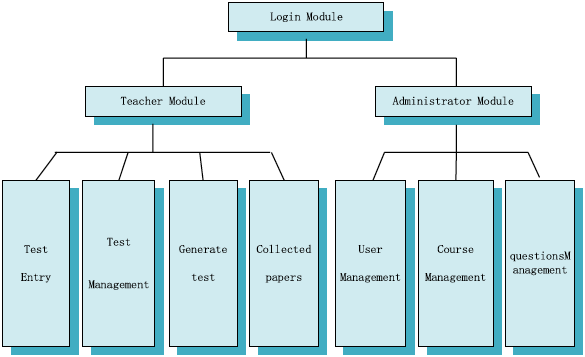
\includegraphics[width=400pt]{Figures/function_module}\\
\caption{Schematic diagram of the system function module \citep{TP-16}} \label{Figure: Schematic diagram of the system function module}
\end{figure}

\begin{figure}[htbp]
\center 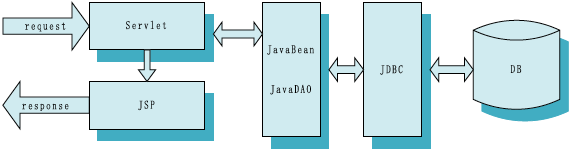
\includegraphics[width=400pt]{Figures/road_map}\\
\caption{Technology road-map of the system \citep{TP-16}} \label{Figure: Technology road-map of the system}
\end{figure}

\begin{figure}[htbp]
\center 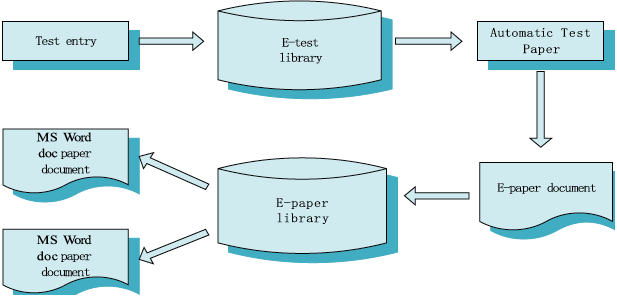
\includegraphics[width=400pt]{Figures/Flow_chart}\\
\caption{Flow chart of the automatic paper generation method \citep{TP-16}} \label{Figure: Flow chart of the automatic paper generation method}
\end{figure}

(Yajuan Zhang, 2011) proposed that although the traditional algorithms in a test paper generation system satisfy the requirements of shuffling the questions. Under certain constraints they do not perform as well as others which have been newly adopted. Here follows a discussion of analysing five intelligent algorithms and how these existing global optimisation algorithms can be integrated into improved shared global optimisation algorithm and dynamic multi branches tree algorithm. These included, improved genetic algorithm, differential evolution algorithm and ant colony optimisation. The particle swarm optimisation algorithm and simulated annealing algorithm. These are divided into two categories which are population evolutionary and others are individual evolutionary and each uses different searching and selection mechanisms. There have been many different studies on trying to improve the algorithms used in terms of speed optimisation however, the improvements were only minor ones. And with the expansion of the system new classifiers need to be constructed for the added samples. The characteristics of the different global optimisation algorithms such as the improved genetic algorithm. Based on the genetic algorithm with modifications such as improvements to integer coding which displays higher search speeds performing well and is very practical. It also avoids prematurity which occurs in the genetic algorithm. The genetic algorithm performs a randomised search simulating natural selection and genetic variation to problem solve. With the disadvantage of having a low search efficiency with premature convergence. The differential evolution algorithm is simple and effective in that the population size remains unchanged throughout the operation process. These operations include variation, crossover and selection with advances such as simple principle, control parameters, robustness a high convergence rate and straightforward realisation. The ant colony algorithm simulates an ant colony and their routing behaviours in nature. Finding a solution through information exchange and cooperation among the ant colony. However, the mechanism for feedback has a slow convergence speed. The particle swarm optimisation algorithm has good performance however, needs to be used indirectly in getting the optimal solution of multiple object optimisation problems. As during a search its own position needs to be updated through a follow up of individual extreme value and global extreme value. Simulated annealing algorithm finds the probability sense using a random search. Which is a global optimisation method.
(Dan Liu, 2013) derived a method for test paper generation through using the ant colony algorithm. A comparison is also made between using other algorithms such as a random variable algorithm a backtracking algorithm and an artificial intelligence algorithm. Describing the random variable algorithm is that is extracts questions and if they meet certain conditions it then forms a test paper based on these conditions. However, it can fail to meet these requirements. Which in turn offers a poor success rate. The backtracking algorithm works well on small scale generation. Once the scale is largely increased so the time taken to process the generation increases. A new approach would be to compose test papers using the ant colony algorithm as it can search at a far greater speed with and intelligent search.
